\documentclass{article}
\usepackage[utf8]{inputenc}
\usepackage{amsmath}
\usepackage{amsmath}
\usepackage[margin=1in]{geometry}
\usepackage{tikz}

\title{Problem Set 5, Question 1}
\author{Samuel Barker, Daniel F. Noriega, Rafeh Qureshi, Tim Schwieg}
\date{November 2018}

\begin{document}

\maketitle

\subsection*{Setup}
There is a society that consumes $O_{total}$ prescription opioids, where individuals with health insurance (these people will be the ones in the government programs) consume $O_i$ opioids and uninsured individuals consume $O_u$ (so that $O_{total} = O_i + O_u$). Between 2001 and 2014, the average out of pocket price of prescription opioids in units of potency fell by a factor of 5. This means that the total expenditures on opioids divided by the amount of opioid-potency consumed decreased. In other words, $\frac{(P_iO_i)+(P_uO_u)}{q(O_{total})}$ decreased by a factor of 5, where $q$ represents the potency of opioids. We assume that the price of opioids acquired through insurance plans is negligible since the problem states that the government makes them ''almost free'', so that $P_i \rightarrow 0$.\par
\vspace{1em}
Prices decreased by a factor of 5 partly because of (1) an increase in the amount of people enrolled in insurance plans, and partly because of (2) an increase in the potency of opioids. Mathematically, these mean that (1) $\frac{O_i}{O_{total}} \uparrow$ and (2) $q_{2001} < q_{2014}$ so in order for the following equality to hold, $O_{0} q_{2001}=O_{1}q_{2014}$, it must be that $O_{0}>O_{1}$.

\subsection*{Model}
To begin, we say that individuals have preferences over $Oq$, which can be thought of as ''opioid-potency'', and $m$--the numeraire (note that we have normalized the price of $m$ to one). Further, since we talked above an ``almost free" price for opioids for insured people, and that this problem is about overdosing, we need some probability of death as a function of $O$ and $q$. This serves two purposes: it creates a causal link between OD rates and opioids in general; and it keeps people from demanding an infinite amount of opioids when facing a price of ``almost" zero.
\\
%SAMUEL BARKER: maybe put back in... "Now, we also wish to model the risk of dying as a result of overdosing on opioids. Thus we say that individuals consume $Oq$ until they get to their optimal level of consumption such that utility is maximized, and one constraining condition is the probability of death."

We say that people have a probability of dying $Pr(\text{death or d=1}) = g(q,O).$  We assume that $g(.)$ is a linear function on $qO$ such that $Pr(death) = \alpha qO$. We further assume that people prefer to have a lower probability of dying (a reasonable assumption, we think). Because of this, there are two things that could constrain consumption of $Oq$: the probability of dying, and the budget constraint. When the following condition is met, then it is the budget constraint that binds:

\begin{align*}
    q\frac{\partial u}{\partial O}+\frac{\partial u}{\partial g(qO)} \frac{\partial g(qO)}{\partial O}>0.
\end{align*}

For the rest of the analysis (until Part C where we will return to this), assume that $P_i$ is small enough for the above equation to \textbf{not bind for insured people} and would \textbf{always hold for uninsured people}.\\

Further, notice that insured people are those that are eligible for a government program that provides cheap health care. We assume that this eligibility is determined by income--the lower income brackets are insured.

\subsection*{Utility Maximization}

First consider the utility of insured people, and uninsured people:

\begin{align}
   & U = f(qO,m) &|& p_iO + m \leq Y_i,\\
   & U = f(qO,m) &|& p_uO + m \leq Y_u.
\end{align}

We have that $p_u > p_i$. Here, by the utility maximizing condition, for each $k\in \{u,i\}$,

\begin{align*}
   q\frac{\partial f(qO,m)}{\partial O} &= \lambda p_k \\
   \frac{\partial f(qO,m)}{\partial m} &= \lambda \\
   O p_u +m &= Y\\
   O p_i + m &= Y.
\end{align*}

They will consume until 

\begin{align*}
   \frac{q\partial f(qO,m)/\partial O}{\partial f(qO,m)/\partial m} = p_k \\
\end{align*}
or until the budget constraint holds, in the case of the uninsured, or until the probability of death binds, as in the case of insured. 

\section*{Part A}
Q: Do you expect opioid price reductions from insurance versus potency to have different effects on opioid deaths?
\\

Now, note that as $\uparrow q$, the utility increases directly through the  utility function. However, as $\downarrow p$, the utility increases indirectly through the expenditure function. Seeing this, we can note that a shift in prices affects \par

\begin{align*}
\frac{\partial f(qO,m)}{\partial \alpha} <0.
\end{align*}

Realize, however, that since we have already said that the probability of death is the constraint that binds insured people's consumption of $qO$, a price fall for insured people would have no impact on their consumption of $qO$--since price falls are only observed by individuals who are not insured, this point does not really change the analysis. Similarly, if $q \uparrow$ with no change in price, an insured person would just choose $O_{after}$ such that $q_{before}O_{before}=q_{after}O_{after}$. \textbf{In both cases, because $qO$ is the same after the shock, the probability of dying is the same as well.}\\

A more interesting case is for the uninsured. Notice for them that our intuition remains correct--lower prices imply greater consumption of $qO$ through greater $O$, and higher potency ($q$) causes greater consumption of $qO$. Thus, we would expect the probability of death to be increasing for uninsured people experiencing these shocks.\\

With these in mind consider the case where the government changes the eligibility requirements for governmental aid for health care. Recall that our motivating difference between insured and uninsured people is income. More people being eligible implies that higher income ranges are included in the insured group than were previously. Call this group (b) in the diagram below:


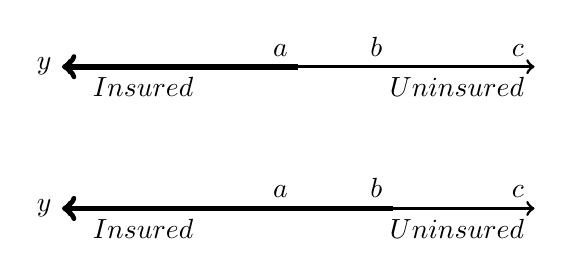
\begin{tikzpicture}[scale=0.6, line width = 1pt]

  \draw[<->] (0,3)--(10,3);
  \draw[<-, line width=.75mm](0,3)--(5,3);
  \node[left] at (0,3){$y$};
  \node[above left] at (5,3){$a$};
  \node[below left] at (3,3){$Insured$};
  \node[above left] at (7,3){$b$};
  \node[above left] at (10,3){$c$};
  \node[below left] at (10,3){$Uninsured$};

  
  \draw[<->] (0,0)--(10,0);
  \draw[<-,line width=.75mm](0,0)--(7,0);
  \node[left] at (0,0){$y$};
  \node[above left] at (5,0){$a$}; left
  \node[above left] at (7,0){$b$};
  \node[above left] at (10,0){$c$};
  \node[below left] at (3,0){$Insured$};
  \node[below left] at (10,0){$Uninsured$};
  
\end{tikzpicture}
\vspace{.2in}

When the average price changes due to more people being induced into having insurance, due to the government regulations, we have only a subset of the population more likely to die due to the change. Namely, take an individual from (a) above. He has the same price $P_i$ and the same preferences for pills $\partial f(qO,m)/ \partial O$, so he consumes the same amount. Similarly, an individual in the portion (c) above, consumes the same amount as before the government change. However, as mentioned in the preceding paragraph, individuals in portion (b) face a decrease in price $P_u - P_i$. We are given that $P_i$ is almost zero and $P_i<P_u$, so people in (b) start consuming more of $O$ and thus are more likely to overdose. Note that since the people of region (a) had consumption that was bounded by the probability of dying--NOT by their budget constraint. If this was true for (a), then it will certainly be true for (b) once they become insured since they presumably have a higher income--their budget constraint would not bind until even later than (a). Thus, all people that have insurance face the same probability of death. Note that small differences could exist for $P_i>0$, but since we have said that $P_i \to 0$, we can say that these differences are arbitrarily small--or, for simplicity's sake, non-existent.\\

In summary, if potency increased and prices remained the same: insured people would consume less $O$ to achieve and equal level of $qO$ as before because they are bound by the probability of dying (which implies that the rate of death remains the same as well); and uninsured people would effectively face a lower price for $qO$ and thus would consume more $qO$ and are therefore more likely to die after an increase in $q$. If more people become insured, then that group of people would face a lower price (which we have said is effectively zero) for $O$ and therefore would be bound by the probability of dying--this obviously implies that more of them would die.\\

Thus we can expect that in either case there would be more overdoses, it is more a question about what populations experience them. In the case where $q$ increases, these deaths would be completely among the uninsured since the insured do not change their consumption of $qO$ (recall that the probability of death is the binding constraint). However, the uninsured could never have a higher death rate than insured people because their consumption of $qO$ would be bound by the probability of dying just as it would for insured people.\\

%Now, when the price changes due to quality, everyone is affected by the change, so individuals in (a), (b) and (c) are all more likely to die due to everyone's increased effective consumption of opioids (as they consume more opioids in terms of potency). Note, here, the increases in consumption (and thus the probability of dying) will be highest for individuals who are already consuming the greatest amount of opioids $O$. However, it is difficult to infer whether this will be individuals who have insurance or people who do not. We could assume that individuals eligible for Government-funded insurance have in general lower income than uninsured individuals. They would face lower prices due to being enrolled in insurance programs, but they would also have a lower income so that in general one would expect them to consume less opioids. Consequently, individuals who have higher income would tend to have a higher change in probability of dying (as they end up consuming more).


\section*{Part B}
Q: Some analysts have argued that, for reasons aside from the price changes noted above, people are consuming more opioids because they are more depressed now (and in 2014) than they were in 2001. If they are correct, what does that say about the price elasticity of demand for opioids?
\\

Note that at the current analysis, individuals with insurance are not changing their consumption of $qO$ as their binding constraint is through their probability of dying with increasing consumption of $q0$, so they would simply decrease $O$ till $q_{2000}O_{2000} = q_{2014}O_{2014}$. With the increased depression, there could plausibly be a reduced disutility to dying, wherein their $ q_{2014}O_{2014}>q_{2000}O_{2000}$. The inelasticity for them of $qO$ would remain the same (i.e perfectly inelastic locally).

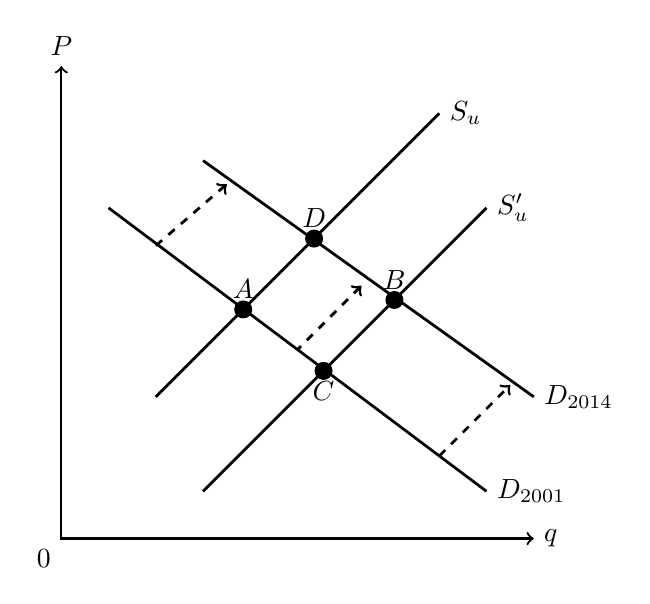
\begin{tikzpicture}[scale=0.6, line width = 1pt]

\draw[thick,<->] (0,10) node[above]{$P$}--(0,0)--(10,0) node[right]{$q$};

\node [below left] at (0,0) {$0$};

\draw (3,1)--(9,7);
\node [right] at (9,7){$S_u'$};
\draw (2,3)--(8,9);
\node[right] at (8,9){$S_u$};

\draw [->,dashed] (8,1.75)--(9.5,3.25);
\draw [<-,dashed] (6.35,5.35)--(5,4);
\draw [->,dashed] (2,6.2)--(3.5,7.5);

\fill (3.85,4.85) circle (.075in);
\node[above] at (3.85,4.85){$A$};
\fill (7.05,5.05) circle (.075in);
\node[above] at (7.05,5.05){$B$};
\fill (5.55,3.55) circle (.075in);
\node[below] at (5.55,3.55){$C$};
\fill (5.35,6.35) circle (.075in);
\node[above] at (5.35,6.35){$D$};

\draw (1,7)--(9,1);
\node [right] at (9,1){$D_{2001}$};
\draw (3,8)--(10,3);
\node [right] at (10,3){$D_{2014}$};

\end{tikzpicture} \par
If changes in consumption were actually attributable to changes other than prices, such as people being more depressed, then it would imply that the price elasticity of demand for opioids is lower than it may have otherwise seemed to be. In other words, demand for opioids would be more inelastic, as it would have been less responsive to price changes than we had previously imagined.\\

We originally imagined that the observed quantity changes were purely due to the price changes. Recall the price changes occurred both due to an increase in the potency of the opioid, which induced individuals to increase their potency-consumption (as the price per unit of potency fell). Additionally, we had the other effect that individuals with a middle income level were shifted from being uninsured to being insured. In calculating the price elasticity of demand for opioids, we would imagine that the entire observed change $\Delta qO = q_{2014}O_{2014} - q_{2001}O_{2001}$ was due to the $\Delta q = q_{2014} - q_{2001}$ and the $\Delta p = p_u - p_i$. However, as the analysts have found, a portion of the change occurred due to the change in the demand for the good. Thus, the change in the consumption of opioids is not completely due to the changes in prices, and partially due to the change in demand itself (driven by individuals being more depressed). Thus, the price is more inelastic than we would have imagined.

$$\epsilon = \frac{\Delta q}{\Delta p} $$

\section*{Part C}
Q: Would your answers to (a) and (b) change if the data showed that opioid deaths among the uninsured increased at the same rate as those who had health insurance?\\

Yes. In our model, insured individuals faced a lower price for opioids than uninsured individuals. As the share of insured people increased in the population, more people had access to cheaper opioids and consequently opioid consumption increased, which resulted in more deaths. In the above analysis, as the prices for individuals in the insured population were low enough, individuals with insurance were not constrained by the prices of the opioids (as these were effectively zero) and were instead constrained by their probability of dying with the increase in $qO$. This required that the change in quality would not move the consumption of potency-weighted pills by insured people, namely $q_{2001}O_{2001} = q_{2014}O_{2014}$ even though $q_{2014}>q_{2000}$\footnote{Thus, trivially implies that $O_{2014}<O_{2001}$ and so individuals would have decreased their consumption of physical pills} and the probability of dying would not change for this population as they were already constrained by $qO$. However, since the change in quality was not binding for the uninsured population (who had a higher $p_u$), the change in quality strictly increased their consumption of $qO$ and strictly increased their probability of dying.\\

However, if the change in the rate of deaths were the same in uninsured and insured groups, this clearly cannot have been the case. Thus, we would come to the conclusion that insured individuals were still constrained by the prices of O, $p_i$ and thus increased their consumption of $qO$ with the increase in potency $q$. More specifically, they increased their consumption of $qO$ by the same proportion that rich individuals increased their consumption of $q0$.\\

Overall, our analysis of (b) remains the same for the insured population as a change in depression still signifies that the change in utility was more attributable to a change in demand as opposed to solely a change in price. This, again, still implies that the demand is more inelastic than we would have previously imagined. However, in this scenario, the price elasticity of consumption of $qO$ is not infinity. Furthermore, the analysis of the insured population would be very similar to the  analysis of the uninsured population.

\section*{Part D}
Q: Part of the cost of using opioids and related products is forgone earnings, e.g., from employment spells that are interrupted temporarily or, as with death, permanently. Moreover, a segment of society has been experiencing reduced foregone earnings. Discuss how the foregone earnings effect might quantitatively compare to the substitution effect you examined in parts (a) and (b). \\

We note that the price of opioids effectively goes down due to the reduced foregone earnings as $p$ decreases to $\tilde{p} = p + cost_{\text{foregone earnings}}$. This would increase the relative consumption of opioids. However, notice that individuals with reduced foregone earnings would also have their income reduced, so the price of foregone earnings will be lower, thereby reducing opioids consumption through an income effect.\\

Let us call the subsection of individuals with reduced foregone earnings $''subsection$ $A''$. These individuals have $\tilde{p_0} = p + cost_{\text{foregone earnings},0}$ and $\tilde{p_1} = p + cost_{\text{foregone earnings},1}$ in periods 0 and 1. Note, however, that the decrease in foregone earnings also implies that their income went from $Y_0$ to $Y_1$ wherein $Y_1<Y_0$.\\

The price of opioids effetively goes down due to the decrease in the reduced earnings, which would increase the amount of opioids consumed if opioids were a normal good. However, there would be an additional effect as individuals' income as a whole decreases. 
Equivalently:

$\epsilon^{M}_{\text{Income Reduction}} = \epsilon^{H}_{\text{Price Increase}} + s_{Opioids}\eta_{Opioids}$

\end{document}
